%!TEX root = cv_ml_notes.tex
% \refstepcounter{chapter}
\chapter{Computer Vision}

\section{Geometric Transformations}

\paragraph{2D Scaling}

$S = \left( \begin{matrix} s_x & 0 \\ 0 & s_y  \end{matrix} \right)$

\paragraph{2D Rotation}

$R = \left(\begin{matrix} \cos  \alpha & \sin \alpha  & 0 \\  -\sin \alpha & \cos \alpha & 0 \\ 0 & 0 & 1  \end{matrix} \right)$

Symmetry group: SO3 vs. SE3

Reflection: Eigenvalues of the rotation matrix contain (-1)

\paragraph{2D Translation} - only possible in homogeneous coordinates

\section{Projective Geometry}

\subsection{Homogeneous Coordinates}

$x = \left(\begin{matrix} u & v & 1 \end{matrix}\right)^T$ pixel space position, only 2 degrees of freedom.

Inhomogeneous coordinates: $x = (\begin{matrix} u & v \end{matrix})^T $

$ x_w = \left( \begin{matrix} x_w &  y_w & w_t & 1 \end{matrix} \right)^T $ world space position

The scale is unknown: $x \mapsto  w x_w$

\subsubsection{Homogeneous Line/Plane Representation}

$ax+by+c = 0 \to (a,b,c)^T p = 0$ for every $p = (x,y,1)$ on the line.

The nice thing about this: for two Euclidean points $p_{1,2} = (x,y,z) $ the line connecting them is given by their cross product: $l = p_1 \times p_2$. 

Similarly, for two lines, their intersection point is given by the cross product: 
$p = l_1 \times l_2$

From homogeneous points to Cartesian image points divide by z. 


\subsubsection{Projection}

A \emph{projectivity} is an invertible mapping $h$ from  to itself such that three points $x_1 , x_2 , x_3$ lie on the same line if and only if $h(x_1), h(x_2 ), h(x_3)$ do:
%
\begin{itemize}
\item check by fitting a line to the point and checking the third point is on the same line
\item line normal coordinates in 3D
\end{itemize}

\subsubsection{Projective Transformation}

From world position $x \in \mathbb{R}^4 \to p \in \mathbb R^3$ pixel homogeneous coordinates. 

Projectivity : colineation :  proj. transformation : homography

A point in an image projected to the world is known up to a scale factor.

\subsection{Transformations Hierarchy (2D)}

\begin{itemize}
\item Projective 8 DoF - co-linearity.
\item Affine 6 DoF - parallelism, ratio of areas, ratio of lengths of parallel lines.
\item Similarity 4DoF - ratios of lengths, angels.
\item Euclidean 3DoF - all of above and scale.
\end{itemize}

% $\left(  \begin{matrix} s\cos  \alpha &  s\sin \alpha  & t_x \\  -s s\sin \alpha & s\cos \alpha & t_y \\ 0 & 0 & 1  \end{matrix} \right)$

% $\left( \begin{matrix} \cos  \alpha & \sin \alpha  & t_x \\  -\sin \alpha & \cos \alpha & t_y \\ 0 & 0 & 1  \end{matrix} \right)$

\subsubsection{Planar Homography}

Relates planar images. Has eight DoFs, can be determined from four point correspondences.
(basically we're estimating the perspective transformation from one plane to another)

From point relations in Euclidean coordinates, can derive a system for the homography. 

This results in a system $Ah = 0$ which is solved using SVD. 
The system is either determined exactly and over-determined, in that case the smallest eigenvalue is a measure of the quality of the fit.

When working with homogeneous coordinates, apply homography to homogeneous coordinates and then divide by $z$.

% Simple Geometric relations using homography:

% Two lines intersection - $l_1,l_2$ - find $x = l_1 \times l_2$  (based on normal equations)

% Line through two points: $l = x_1 \times x_2 $

\paragraph{Homography Line Transformation}

$l^\prime = \mathbf{H}^{-T} l$

\textbf{Ideal Points} - intersection points of parallel lines

\subsection{3D Homography}

Plane normal equation: $ax_1 + bx_2 + c_x3 + d x_4 = 0$ 

If $\pi^T p = 0$ the point lies on the plane / the plane passes through the point

We can fit a plane to three points by solving:
$\left( \begin{matrix} x_1^T \\ x_2^T \\ x_3^t \end{matrix} \right) \pi = 0 $

\subsection{Cameras and Image Formation}

The camera model relates pixels and rays in space

Optical axis - usually denoted as $z$, faces into the world.
The optical axis passes between the camera origin and the principal point in the image.

Principal point - the point at which the principal axis passes through the image plane.

Image plane - can be visualized in front of the sensor, the formulation is equivalent.


\subsection{Perspective Camera Model}
The camera matrix projects from the world space to image space. Using homogeneous coordinates allows for translation.

The actual image plane is actually only a few mm wide.

Central Projection Model

\subsection{Camera Intrinsic $K$}
$K = \left( \begin{matrix} 
\alpha_x & \gamma & u_0 & 0 \\
0 & \alpha_y  & v_0 & 0 \\
0 & 0 &  1 & 0 \\
\end{matrix}
\right) $

The camera model has five intrinsic parameters:
\begin{itemize}
\item $f$ - focal length
\item  image sensor format - $m_x$ and $m_y$ are the pixel dimensions
\item  $\gamma$ skew coefficient between x-y
\item  $(u_0,v_0)$ *principal point*, usually in the middle of the sensor
\item  $\alpha_x = f m_x $
\item  $\alpha_y = f m_y $
\end{itemize}

This model cannot represent lens distortion. Usually the model is simplified to:

$ K = \left( \begin{matrix} 
f & 0 & h/2 & 0 \\
0 & f  & w/2 & 0 \\
0 & 0 &  1 & 0 \\
\end{matrix}
\right) $

\subsection{Camera Extrinsic Parameters $R,T$}

$ \left[ 
\begin{matrix} 
R_{3x3} & T_{3x1} \\
0_{1x3} & 1 
\end{matrix}
\right] $

The extrinsic parameters define the position of the camera center and the camera's heading in world coordinates. $T$ is the position of the origin of the world coordinate system expressed in coordinates of the camera-centered coordinate system. 

The actual camera position in world coordinates is $C = -R^{-1}T=-R^{T}T $

\subsection{Camera Intrinsic Estimation}

For capturing a planar object:

\begin{enumerate}
\item Set the planar object as the infinity plane: $x = ( \begin{matrix} x_1 & x_2 & 0 & 1 \end{matrix})^T$
\item Estimate the transformation for each point using homography relations: $ x \times H x = 0$ resolves to a series of equations that can be solved for h.
\item Normalize the points: translate points s.t. centroid is at origin, and perform isotropic transformation- mean distance from origin of $\sqrt 2 $. 
\item Minimize the 2 sided reprojection error - from $img1 \leftarrow img2$ and from $img2 \leftarrow img1$
\item This relates to the maximum likelihood estimate:
	Given $n\ge 4$ 2D to 2D point correspondences {$x_i\leftrightarrow x_i\prime$}. 
	Determine the Maximum Likelihood Estimation of $H$ (this also implies computing optimal $x_i^\prime=Hx_i$) 
\end{enumerate}

To perform the last step: 
(i) Initialization compute an initial estimate using normalized DLT or RANSAC
(ii) Geometric minimization of symmetric transfer error: 

Minimize using Levenberg-Marquardt over 9 entries of $h$ or reprojection error:
- compute initial estimate for optimal $x_i$
- minimize cost over ${H,x1,x2,...,xn}$
- if many points, use sparse method

\subsubsection{Other Considerations}
\begin{itemize}
\item Radial lens distortion
\item Rolling shutter effects
\end{itemize}

\section{Image Features and Matching}

\textbf{Local features} - compact description of image regions.

\textbf{Detectors} are used to find salient structures in images. Common salient structures include corners, blobs
and keypoints.

A \textbf{descriptor} is a compact representation of the image region around that keypoint. (Good) Descriptors allow to establish matches between images by descriptor comparison and for subpixel localization.

\subsection{Invariant Descriptors \& Matching}

Feature matching: extract features independently and match by comparing descriptors.

Feature tracking: extract at first frame, find same feature in the next frame

Image features may go through the following transformations:

Geometric transformations:
\begin{itemize}
\item Translation, rotation, scaling
\item Perspective foreshortening 
\end{itemize}

Photometric transformations:
\begin{itemize}
\item Non-diffuse reflections 
\item Illumination
\end{itemize}

Good descriptors and detectors are invariant to these transformations. 

\textbf{Desirable Properties}
\begin{itemize} 
\item Precise (sub pixel) localization
\item Repeatable detections under rotation, translation, illumination, perspective distortion.
\item Detect distinct/salient features
\end{itemize}

Feature Points - distinct points in image (i.e. corners)

\section{Feature Detection}

/TODO - all of the data in this part of the document was lost due to a bug in the text editor. Redo.

\subsection{Harris Corner Detector}

Stable image features should maximize the uniqueness of the region, which is measured by auto-correlation.

$$ 
\mathbf{A} = \left(  \begin{matrix} I_x^2 &  I_xI_y \\
I_xI_y & I_y^2
\end{matrix} \right) $$

\begin{itemize}
\item Cornerness depends on the eigenvalues $\lambda_1,\lambda_2$ of the auto-correlation matrix.
\item Homogeneous - both small.
\item edge: one large, one zeroish.
\item corner: both large.
\end{itemize}

Choosing local maxima as keypoints. 

Subpixel accuracy by fitting quadratic 

Variant to affine and scale transformation.

\subsection{SIFT Features}

SIFT - Scale invariant image transform.

Difference of Gaussians generates candidates. 
Consider local extrema in scale and spatial space.
Invariant to translation, rotation and scale.
Quad fit for sub-pix accuracy.

Orientation Assignment
\begin{itemize}
\item  Compute gradient for each pixel in patch at selected scale
\item  Bin gradients in histogram \& smooth histogram
\item  Select canonical orientation at peak(s)
\item  Keypoint = 4D coordinate 0 (x, y, scale, orientation)
\end{itemize}

\subsection{Affine Invariant Features}
Scenario - extreme wide baseline matching

Maximally Stable Extremal Regions (MSER)

Detects extremal regions which are brighter / darker than surrounding
Region is a connected component
Compute its centroid + PCA
Fit ellipse to canonical circle
Compute orientation and re-orient in canonical space.

\subsection{Lowe's SIFT Descriptors}

Local descriptors based on gradient magnitude and orientation.

Ignore pixel values, use only local gradients

Gradient direction more important than positions

Partition into sectors to retain spatial information

Thresholded image gradients are sampled over 16x16 array of locations in scale space

Create array of orientation histograms

8 orientations x 4x4 histogram array = 128D

Descriptor size was chosen based on careful parameter tuning. 


\textbf{Hard vs. Soft Binning}

Hard binning results in discontinuous descriptors with small changes.

Soft binning - gradual changes to descriptor.

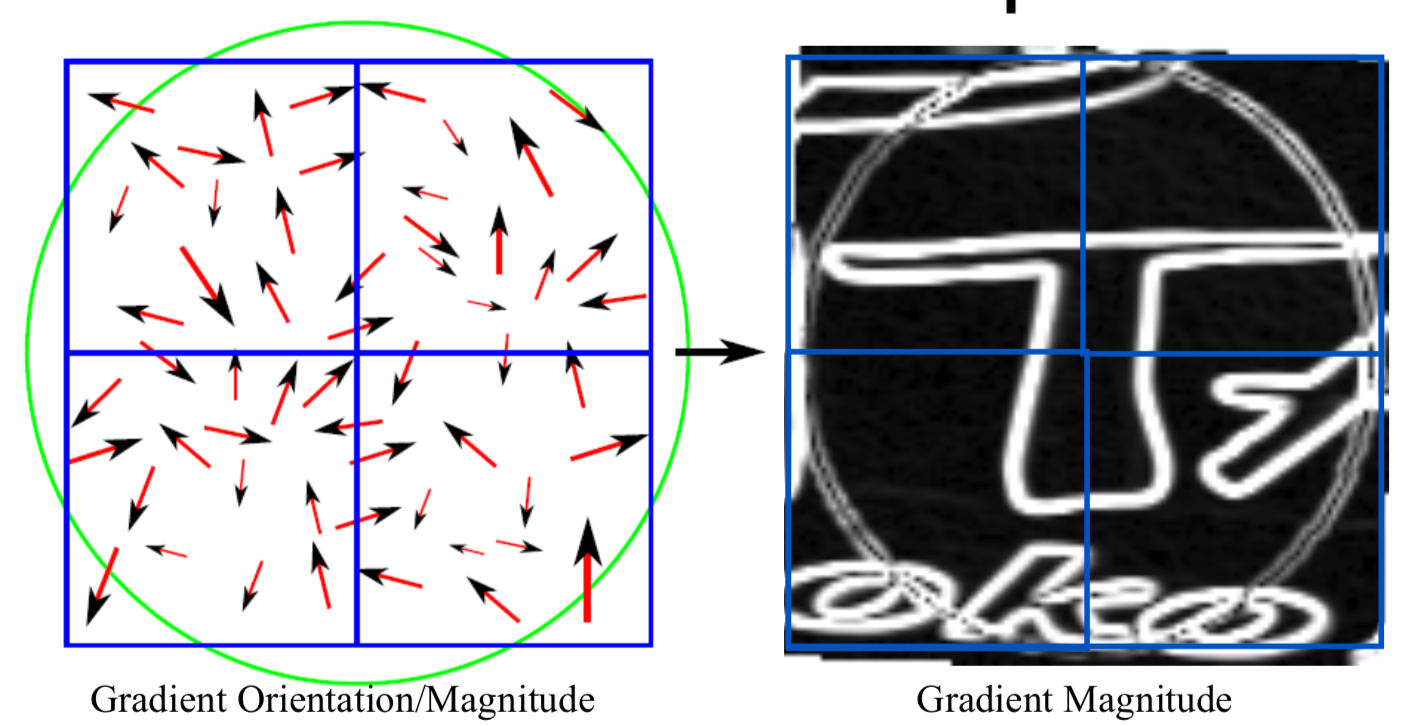
\includegraphics[width=0.9\columnwidth]{cv_figures/lowe.png}

\section{Feature Matching}

Comparing image descriptors

\subsection{ Similarity Metrics for Patch/Line Matching}

\paragraph*{ SSD - Sum of Squared Distances}

$SSD = \sum_x \sum_y (I(x,y) - I^\prime(x,y))^2$

Only translation invariant.

$MSD=\frac{1}{2xy} \sum_{i,y}\left|P_{x,y}^{(i)} - P^{(j)}_{x,y}\right|^2$


\subsubsection{Zero-Mean Normalized Cross Correlation}
Consider two real valued functions  $f,g$  differing only by an unknown shift along the x-axis (i.e. disparity). One can use the cross-correlation to find how much $g$ must be shifted along the x-axis to make it identical to $f$ 

The probability density of the difference $Y-X$ is formally given by the cross-correlation.

The formula essentially slides the $g$ function along the x-axis, calculating the integral of their product at each position.

$$ NCC = \frac{N(I^\prime,I)}{\sqrt{N(I,I)N(I^\prime,I^\prime)}} $$
$$ N(I^\prime,I) = \sum_{xy} (I(x,y) - \bar I )(I^\prime(x,y) - \bar I^\prime ) $$

This works for uniform illum. changes
But even this is still fragile (i.e. non uniform changes)

\subsection{Binary Descriptors}

SIFT is powerful descriptor, but slow to compute
\begin{itemize}
\item Faster alternative: Binary Descriptors:
\item Idea: Compute only sign of gradient
\item Efficient test: Compare pixel intensities
\item Random comparisons work already very well
\end{itemize}

\textbf{Pros}
\begin{itemize}
\item Efficient computation
\item Efficient descriptor comparison via Hamming distance (1M comparison in ~2ms for 64D)
\end{itemize}

\textbf{Cons}
\begin{itemize}
\item Not as good as SIFT / real-valued descriptors
\item Many bits rather random = problems for efficient nearest neighbor search
\end{itemize}


\subsection{Feature Matching}

Spatial Search Window:
\begin{itemize}
\item Requires/exploits good prediction
\item Can avoid far away similar-looking features
\item Good for sequences
\end{itemize}

Descriptor Space:
\begin{itemize}
\item Initial tree setup
\item Fast lookup for huge amounts of features
\item More sophisticated outlier detection required
\item Good for asymmetric (offline/online) problems, registration, initialization, object recognition, wide baseline matching
\item Huge memory demands
\end{itemize}



\subsection{Feature Tracking}

Identify features and track them over video

Small difference between frames

Potential large difference overall

\subsection{KLT - Kanade Lukas Tomasi}
\begin{itemize}
\item Using the auto-correlation matrix, assumption that the motion is small.
\item Linearize and solve.
\item Multi scale (coarse to fine), iterate and refine over all image scales.
\item Assumes brightness constancy.
\end{itemize}

\textbf{Problem}  Affine model tries to deform sign to shape of window, tries to track this shape instead. 
\textbf{Solution} Perform affine alignment between first and last frame, stop tracking features with too large errors. 

\subsubsection{Aperture Problem}

Assumption: neighbors have same displacement

\subsubsection{Summary}
Motivation: Exploit small motion between subsequent (video) frames

Key ideas:
- Brightness constancy assumption
- Linearize complex motion model and solve iteratively
- Use simple model (translation) for frame-to- frame tracking
- Compute affine transformation to first occurrence to avoid switching tracks


\section{Stereo Vision}

Two cameras, $C_L$ and $C_R$

Their respective optical centers $O_L$ and $O_R$

The world space point $X$ and its projection in each one of the cameras: $x_L, x_R$

\subsubsection{Epipolar Point}

The epipolar points $e_L, e_R$ are defined as the points where the baseline intersects each one of the camera images, or the center of each camera as projected into the other cameras image.

\subsubsection{Epipolar Line}

A line segment between the epipolar point and the projection of the X on the image.

A second epipolar line segment is the projection of this line onto the first camera image plane

A point in one image generates a line in the other on which its corresponding point must lie

\subsubsection{Epipolar Plane}

A plane that passes through both camera centers.

\subsection{Essential Matrix}

For two points in two images of a camera stereo pair which correspond to the same $3D$ world position, the following is true: 
$\mathbf{y}^{\prime T}\mathbf{Ey}=0$

This relates the two calibrated cameras.

The essential matrix can be seen as a precursor to the fundamental matrix. 

The essential matrix can only be used in relation to calibrated cameras, it requires known intrinsic camera parameters (for normalization).

The essential matrix can be useful for determining both the relative position and orientation between the cameras and the 3D position of corresponding image points.

 E is an essential matrix iff two of its singular values are equal, third is 0.

$\mathbf{E}=\mathbf{RS}$

where 

$\mathbf{S} = \left( \begin{matrix} 0 & -T_z & T_y \\ T_z & 0 & -T_x \\ -T_y & T_x & 0  \end{matrix} \right)$

weird transformation matrix with 3 DoF and R also has 3 DoFs

rank 2 

Has both left and right nullspaces.

Depends only on extrinsic parameters

\subsection{ Fundamental matrix}

$\mathbf F \in \mathbb{R}^{3\times3} = \mathbf{M}_r\mathbf{RSM}_l^{-1}$ 

The Fundamental matrix relates corresponding points in stereo images.
$\mathbf{X}^{\prime T}\mathbf{Fx}=0$ and $\mathbf{F}_{3x3}$

Analogous to essential matrix. The fundamental matrix relates pixels (points) in each image to epipolar lines in the other image.

It is related to the essential matrix $\mathbf{E} = \mathbf{K}^{\prime T} \mathbf{FK}$ where $\mathbf{K}^{\prime}, \mathbf{K}$ are in the intrinsic matrices of both cameras.

$rank(\mathbf{F}) = 2$

\textbf{Here a bunch notes were deleted.}

\subsection{Eight Point Algorithm}

\url{https://en.wikipedia.org/wiki/Eight-point_algorithm}

From homography relation $x^\prime F x = 0$, $F$ is rank 2, has seven DoF. 

Eight points define a linear system, which is it contains no errors, can be solved as SVD and the smallest column of V defines F.

Otherwise this is solved in the least square sense and one computes a $F^\prime$ which is most similar to F and also $\|F\|=1$. Usually compute SVD for F and drop the smallest eigenvector. 

Since the whole algorithm is numerically sensitive, all points and matches need to be normalized. 

\subsection{Singularity Constraint - Seven Point Algorithm}
From 7x9 matrix, compute eigenvalues.
Solve up to $F = \alpha F_1 + (1-\alpha) F_2$
Enforce a constraint by: $\det(F) = 0$ (cubic in $\lambda$)
cubic in $\alpha$ => 1 or 3 solutions.

\subsection{Five Point Algorithm}

For the calibrated case, only compute $\mathbf{E}$

Generate a $5\times9$ matrix for 9 entries of $\mathbf{E}$

$4D$ solution space, w = 1 reduces one dimension.

10 cubic polynomials generated from 
Perform Gauss-Jordan elimination on polynomials.

\subsection{Automatic Computation of $\mathbf{F}$}
1. Extract features
2. Compute a set of potential matches
3. Robust estimation of $\mathbf{F}$ via RANSAC  
4. Compute $\mathbf{F}$ based on all inliers
5. Look for additional matches
6. Refine $\mathbf{F}$ based on all correct matches

\subsection{Robustness to False Matches - RANSAC}

Number of samples requires depending on dataset size and \# of inliers for high certainty that the samples contains an inlier set:
$\eta = 0.01$

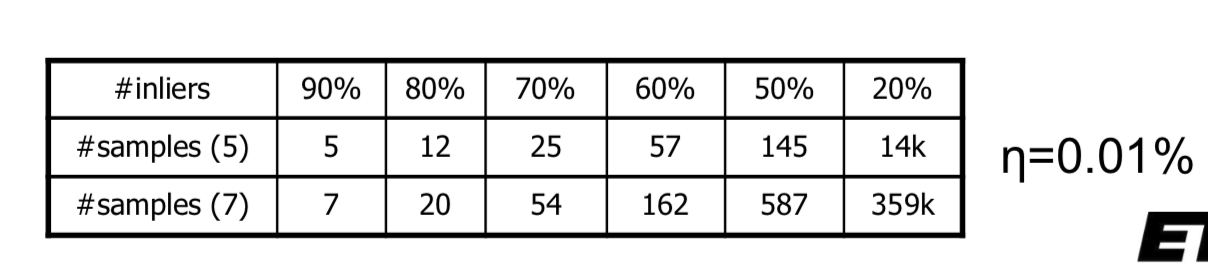
\includegraphics[width=0.9\columnwidth]{cv_figures/ransac.png}

Restricted search around epipolar line (e.g. $1.5$ pixels)
Relax disparity restriction (along epipolar line)

\section{Structure From Motion}
\subsection{Sequential / Incremental SfM}

\begin{enumerate}
\item  Initialize Motion
\item  Initialize Structure
\item  Extend Motion
\item  Extend Structure
\item Repeat 3-4
\end{enumerate}

Initialize:
\begin{itemize}
\item Compute pairwise epipolar geometry
\item Find pair to initialize structure and motion
\item Repeat:
\item For each additional view
\item Determine pose from structure 
\item Extend structure
\item Refine structure and motion
\end{itemize}

Recap Essential matrix:  $E=[t]\times R$

\begin{itemize}
\item  Motion for two cameras: $[I|0], [R|t]$
\item Essential Matrix decomposition: $E= U \Sigma V^T$
\item Recover $E$ and $t = \pm u^3$ and $R=UWV^T or R=UW^TV^T$
\item The equation has four solutions, but only one is meaningful. 
\end{itemize}


Generate hypothesis using 6 points (two equations per point) - planar scenes are degenerate!

Stereo Constraints and their implications:
\begin{itemize}
\item 1-D Epipolar Search -  Arbitrary images of the same scene may be rectified based on epipolar geometry such that stereo matches lie along one dimensional scanlines. This reduces the computational complexity
and also reduces the likelihood of false matches.
\item Monotonic Ordering  -Points along an epipolar scanline appear in the same order in both stereo images, assuming that all objects in the scene are approximately the same distance from the cameras.
\item Image Brightness Constancy - Assuming Lambertian surfaces, the brightness of corresponding
points in stereo images are the same.
Match Uniqueness For every point in one stereo image, there is at most one corresponding point in the other image.
\item Disparity Continuity - Disparities vary smoothly (i.e. disparity gradient is small) over most of the image. This assumption is violated at object boundaries.
\item Disparity Limit - The search space may be reduced significantly by limiting the disparity range, reducing both computational complexity and the likelihood of false matches.
\item Fronto-Parallel Surfaces - The implicit assumption made by area-based matching is that objects have fronto-parallel surfaces (i.e. depth is constant within the region of local support). This assumption is violated by sloping and creased surfaces.
\item Feature Similarity - Corresponding features must be similar (e.g. edges must have roughly the same length and orientation).
\item Structural Grouping - Corresponding feature groupings and their connectivity must be consistent.
\end{itemize}

\textbf{Photometric issues:} specularities, strongly non-Lambertian BRDF’s.
\textbf{Surface structure:} lack of texture, repeating texture within horopter bracket
\textbf{Geometric ambiguities:} as surfaces turn away, difficult to get accurate reconstruction
(affine approximate can help); at the occluding contour, likelihood of good match but incorrect
reconstruction. 

\textbf{Motion Initialization:} Cheirality Constraint

\subsection{Global SfM}

SfM approaches often work on an unordered set of images. Often computed in the cloud with little to no time constraints.

One of the challenges in SfM is to retrieve near-by images, and add images one by one to a growing graph while accounting for potential outlier images so that robust reconstruction maybe performed. (i.e. Building Rome in a Day also talked a lot about system design).

Initialize: Compute pairwise epipolar geometry

Compute:
\begin{itemize}
\item Estimate all orientations
\item Estimate all positions
\item Triangulate structure
\item Refine structure and motion (bundle adjustment)
\end{itemize}

Pros: More efficient, more accurate 

Con: Less robust




SFM might be employed on a huge set of potential images. It's a challenge to retrieve near-by images, and add images one by one to a growing graph while accounting for potential outlier images so that robust reconstruction maybe performed. 

\section{Dense Correspondences and Stereo Matching}

\subsection{Triangulation}


\subsection{Disparity}
Definition: difference in image location of the same 3D point between stereo images

Task: construct 3D model from 2 images of a calibrated camera.

\begin{enumerate}
\item Find corresponding points
\item Estimate epipolar geometry
\item Rectify images
\item Dense feature matching
\item 3D reconstruction
\end{enumerate}

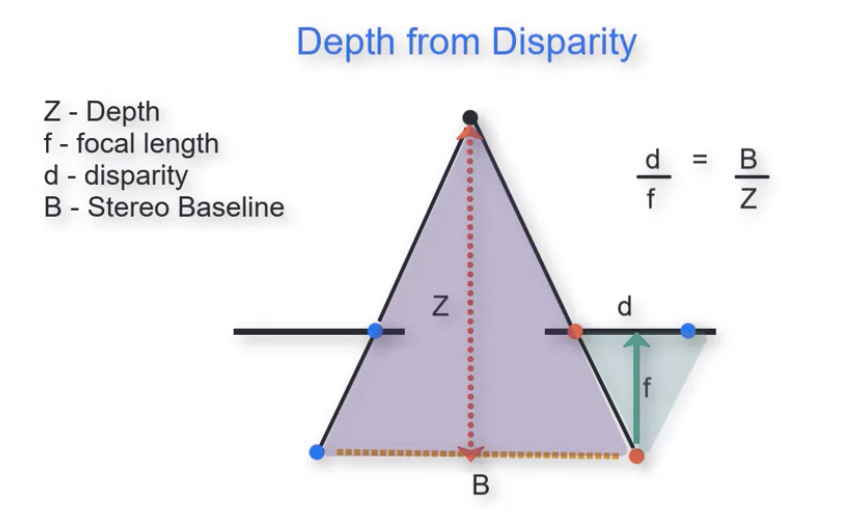
\includegraphics[width=0.75\columnwidth]{cv_figures/disparity.png}

Baseline - dist. between camera centers
\begin{itemize}
\item $f$ - focal length
\item $d$ = disparity between the points
\item $z$ = dist from object
\end{itemize}

From triangle similarity: $\frac{B}{z} = \frac{d}{f}$

Looking at this relationship in depth:

${d}=\frac{Bf}{z} $

$\frac{dd}{dz}=-\frac{Bf}{z^2}$

$dd = \frac{f}{B}dz$

$\Delta z = \frac{Z^2}{Bf}dd$

$(x^\prime,y^\prime)=(x+D(x,y),y)$

Depth resolution is better when the camera is closer to the objects.

The disparity between two points in a stereo pair is inversely proportional to their distance from the observer.


\subsection{Multiple View Geometry - Single Center of Projection}

Three camera views are related via a trifocal tensor 

Having multiple cameras close together results in better depth resolution, less noise, etc.

\subsection{Rectification}

Pre-warping images such that the corresponding epipolar lines are coincident

For a rectified image pair:

\begin{itemize}
\item All epipolar lines are parallel to the horizontal axis of the image plane
\item Corresponding points have identical vertical coordinates.
\end{itemize}

Rectification can be done for image pairs, but may prove impossible for a collection of random cameras, unless they are "parallel" of some sort

How to compute rectification?

1. Rotate both cameras s.t. they're perpendicular to the line connecting both camera centers - using the smallest rotation possible and relying on the freedom of tilt. 
2. To determine the desired twist around the optical axes, make the up vector perpendicular to the camera center line -> the corresponding epipolar lines are horizontal and the disparity for points at infinity is 0. 
3. Rescale images if necc.

Then the pixel matching can be done for a single dimension on every scanline - reduces the dimensionality of the problem to 1D search

\subsubsection{How does it look in math?}

Assuming one camera is $K = [ I 0]$

\yk{TODO}

\subsection{Assumptions for Stereo Matching}

- Small baseline
  - Lower precision and higher correspondences  / similar appearance
- Most scene points are visible in both images
- Image regions are similar in appearance

Left view images will move to the left in the right image - optimization by maximizing normalized cross-correlation.

\textbf{Uniqueness Constraint} 
In an image pair each pixel has at most one corresponding pixel, if occlusion none.

Block matching has an assumption about frontal view.

\subsection{Graph Cut}

\textbf{Treats Stereo Matching as Energy Minimization}

Data term + disparity smoothness term (x) + disparity smoothness term (right)

NP-hard using graph cuts or belief propagation (2-D optimization)

Instead do dynamic programming along many directions
Don’t use visibility or ordering constraints
Add costs of all paths

\textbf{Patch Match Stereo}


\section{Stereo Reconstruction Pipeline}

\subsection{Stereo Photogrammetry}

Small vs large baseline:

Robust binocular stereo
Point matching
adaptive point-based filtering of the merged point clouds, and efficient, high-quality mesh generation.

\subsubsection{Bundle Adjustment}

Bundle adjustment amounts to jointly refining a set of initial camera and structure parameter estimates for finding the set of parameters that most accurately predict the locations of the observed points in the set of available images. 

The assumption is that image measurements are noisy then the equations $x_i = P_i X$ will not be satisfied exactly. 

Bundle adjustment is a maximum likelihood solution (maximizes the probability of the model) under Gaussian  noise assumption. 

We wish to estimate projection matrices $P^i$ and $3D$ points $X_j$ which project exactly to the image point $x^{ij}$ as $x^{ij} = P^i X_j$ and also minimize minimize the image distance between the reprojected point and detected (measured) image points $x^{ij}$ for every view in which the 3D point appears,

Input: $n \; 3D$ points, $m$ views, $x_{ij}$ is the projection of the $i$th point on image $j$. $v_{ij}$
This estimation involving minimizing the re-projection error 

$\min \sum_{i,j} d(P X^j, x_j^i)^2 $ in image space.

\url{https://wikimedia.org/api/rest_v1/media/math/render/svg/c3d1bb3a51f8bafc07c30a99c3f3f15e008d0259}
 denote the binary variables that equal 1 if point $i$ is visible in image $j$. Assume also that each camera $j$  is parameterized by a vector $\mathbf{a}_{j}$ and each 3D point $i$ by a vector $\mathbf{b}_{i}$ . 

Bundle adjustment minimizes the total re-projection error with respect to all 3D point and camera parameters, specifically

It's advantages: tolerant to missing data (sum), while providing a true ML estimate. 
Allows assignment of individual covariances to each measurement
may also be extended to include estimates of priors and constraints on camera parameters or point positions

Cons:
requires a good initialization 
can become an extremely large minimization problem (solution: use last N (key)frames)

Iterative minimization:

Since each camera has 11 degrees of freedom 
Each 3D space point 3 degrees of freedom

n points over m views requires minimization over $3n + 11m$ parameters. 

For Levenberg–Marquardt algorithm the matrix dimensions are $(3n + 11m)\times (3n + 11m)$. 

Factorizing this is on the scale of expensive to infeasible. Strategies including interleaving (block coordinate descent) camera and geometry optimization and limiting the observations.

ML Bundle Adjustment for Affine Camera Model

\begin{figure}[h]
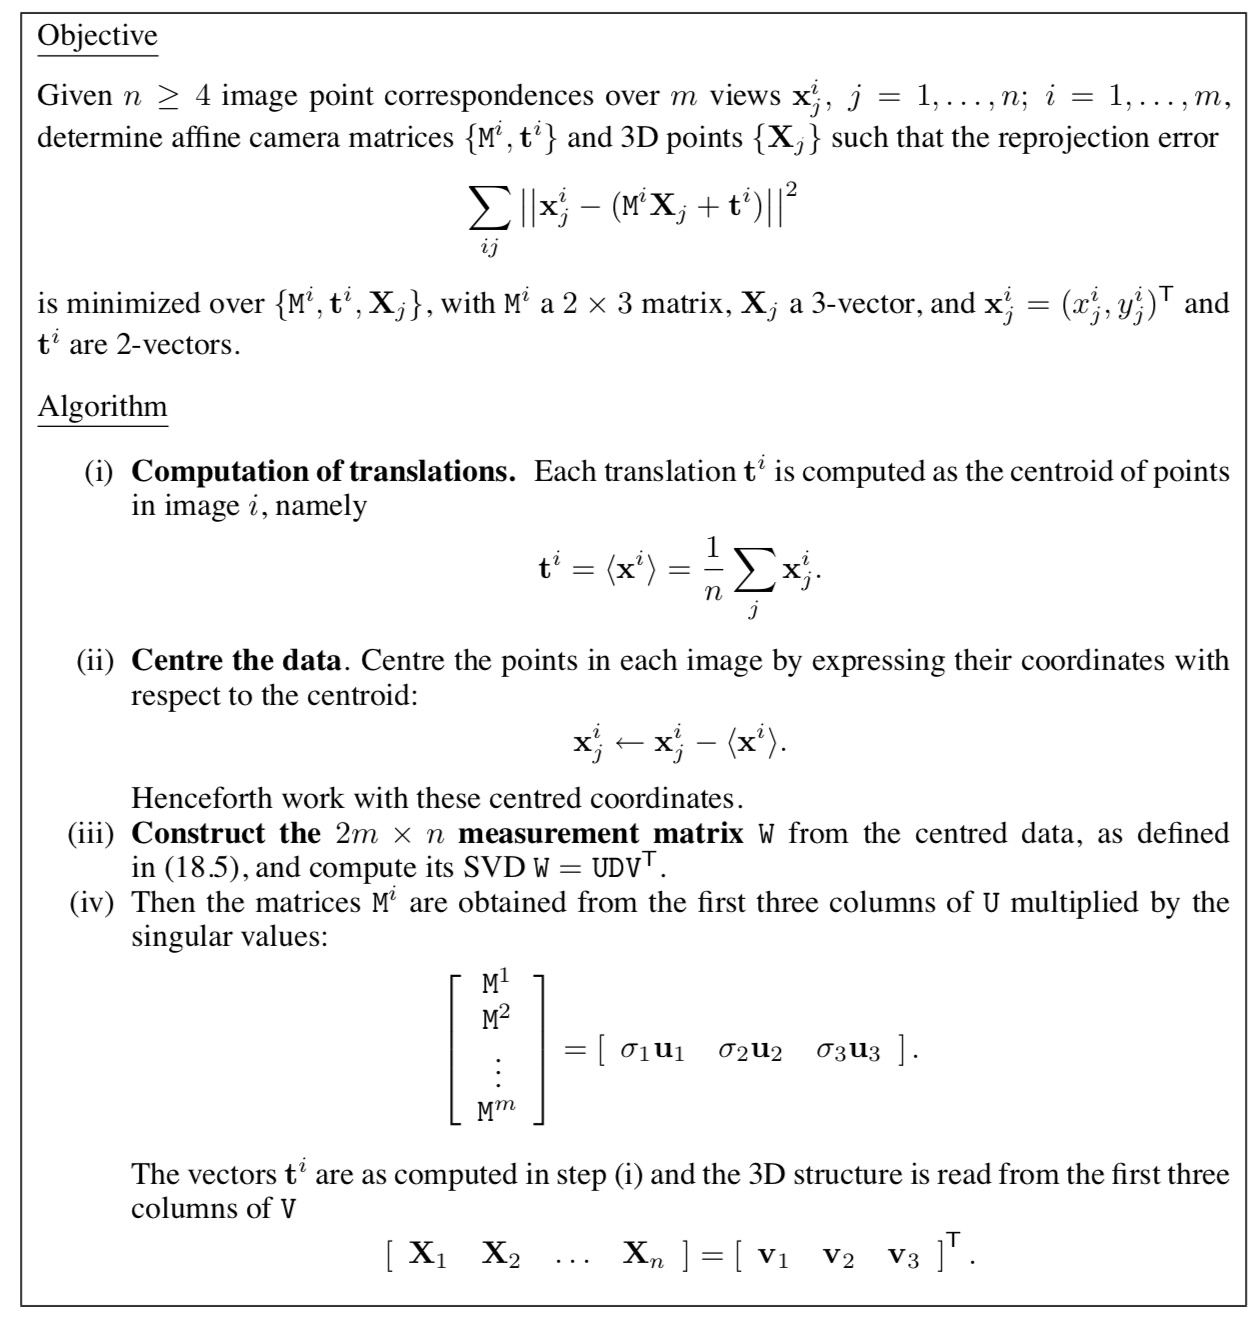
\includegraphics[width=1.0\columnwidth]{cv_figures/ml_bundle.png}
\caption{Source: Multiple View Geometry}
\end{figure}

$\min _{{{\mathbf  {a}}_{j},\,{\mathbf  {b}}_{i}}} \sum _{{i=1}}^{{n}}\; $
$ \sum _{{j=1}}^{{m}}\;v_{{ij}}\,d({\mathbf  {Q}}({\mathbf  {a}}_{j},\,{\mathbf  {b}}_{i}),\;{\mathbf{x}}_{{ij}})^{2}$

where $\mathbf {Q} (\mathbf {a} _{j},\,\mathbf {b} _{i})$ is the predicted projection of point $i$ on image $j$ and $d(\mathbf {x} ,\,\mathbf {y} )$  denotes the Euclidean distance between the image points represented by vectors $\mathbf{x,y}$

Bundle adjustment is tolerant to missing image projections 

Minimizes a physically meaningful criterion

This is typically solved using Levenberg–Marquardt Algorithm

When solving the minimization problems arising in the framework of bundle adjustment, the normal equations have a sparse block structure owing to the lack of interaction among parameters for different 3D points and cameras.

\paragraph{Levenberg–Marquardt}

Here the idea is that the energy terms are separable, and when structured in a matrix we have a distinct block structure with a diagonal block which depends on position only. 

Computing its inverse is easy, which allows to solve for a correction in positions, which then reduce the problem of the solving the correction to the camera parameters to solving a smaller linear system.

The normal equation is then solved by Cholesky factorization, as the matrix is not necessarily invertible and its inverse is not sparse.

\paragraph{Cost Function}
LM requires a cost function which is robust to outliers. 
LS assumes a Gaussian noise distribution and independent observations, this will lead to poor convergence in the presence of any outliers. 

Using a Cauchy or Huber loss is more robust.

\paragraph{Reconstruction from Sequences}

There is an ordering on the images
Small baseline - easy to identify correspondences, both in appearance 

The disadvantage of a small baseline is that the 3D structure is estimated poorly. However, this disadvantage is mitigated by tracking over many views in the sequence so that the effective baseline is large.


\paragraph{Feature Tracking}

Over the sequence, have to think about how the appearance of the feature changes.
Inc. updating the features can cause to drift in localization and introduce error, while affine mapping to a keyframe at every step is also not likely to work.


\subsubsection{Surface Reconstruction}

\begin{itemize}
\item Match points and compute depth field
\item Approximate normals i.e. approximating the planarity from the point neighborhood
\item  Reconstruct surface - for example, fit planes, or Poisson surface reconstruction
\end{itemize}

\section{Bundle Adjustments and SLAM}

Refinement step in Structure-from-Motion.

Produce jointly optimal 3D structures $P$ and camera poses $C$.

Minimize total re-projection errors $z$.

The cost function $\operatorname{argmin}_X \sum_i \sum_j \Delta z_{ij}^T W_{ij} \Delta z_{ij} $

$W_{ij}$ : Measurement error covariance
$X = [P,C]$


\paragraph{Minimization Techniques}

\begin{itemize}
\item GD - slow convergence near minimum
\item Newton method - second order approx, requires inverse Hessian computation - expensive
\item Gauss - Newton - estimate the Hessian $H = J^TWJ$ and solve using normal equation - might get stuck and slow convergence 
\item Levenberg-Marquardt - Regularized Gauss-Newton with damping factor. 
$\lambda \rightarrow 0$: Gauss-Newton (when convergence is rapid)
$\lambda \rightarrow \infty$ Gradient descent
\end{itemize}

Solving the normal equation can be computationally inefficient. Schur-Complement technique is used to accelerate the computation. 

While $A$ is sparse, but $A^{-1}$ is not, therefor use sparse matrix factorization to solve system. 
Optional factorizations: LU, QR or Cholesky.

Visual SLAM works in real-time on an ordered sequence of images acquired from a fixed camera set-up (i.e. one or two particular cameras). 
large scale visual SLAM is typically restricted to trajectories of a few kilometers.

SfM approaches often have to work on an unordered set of images often computed in the cloud with little to no time constraints and might employ different cameras, have been scaled to work on the “planet” level. 

Bundle adjustment (BA), pose-graph optimization (BA without optimizing for 3D points, or motion-only BA), or more generally some sort of non-linear optimization is employed in many state-of-the-art SLAM systems. 

BA is expensive, in SLAM there isn't enough computational budget to run BA on all frames - usually only performed on last N (key)frames. 

SLAM approaches try to cut corners when it comes to feature descriptors and matching, really every stage of the pipeline, to ensure real-time performance in a budget.

In visual SLAM, this problem is just not there since you have an ordered set - you know that neighboring images are expected to heavily overlap with each other - making the problem easier.

\subsubsection{SLAM with Depth Sensors}

It isn’t quite correct to say you avoid the correspondence problem, but the depth information is a big advantage. One common approach is to use the iterative closest point algorithm to align the next depth map to the previous one (or to the map you are building up over time in the case of SLAM), which works when the frame-rate is high enough to expect overlap between every depth-map and for the initialization to be close enough to the correct answer to converge. This way you find correspondence between all the points at once in 3D space, without the difficult search associated with feature matching between RGB images.

\subsubsection{Loop Closure / Relocalization}
In Visual SLAM, the robot/camera begins from the origin and explores its environment while keeping a record of its location with respect to the origin (odometry) and creating a sparse or dense map of the environment. A perfect odometry (visual?) would solve the visual SLAM problem without ever requiring another essential component of the SLAM system, that is, visual place recognition.

Visual Place Recognition is an integral and common part of both Relocalization and Loop Closure in visual SLAM. The idea is to parse the entire database of images and find the best matching hypothesis for the current image. This implies that for both relocalization and loop closure, it is a mandatory condition that the current image is actually a revisited place and we have a matching reference image stored within our database.

So, when do we need Relocalization?

As the name suggests, it is a re-localization, that is, the robot in its current state is no more aware of its location within the map. This generally happens when visual odometry fails, that is, the robot is unable to track its pose/position due to lack of sufficient matching between the current and recent previous images. Therefore, visual place recognition is called for help and after finding a confident match from within the entire database, the robot pose is re-estimated with respect to the map.

What about Loop Closures?

The primary purpose of loop closures is to overcome the drift accumulated in the robot trajectory over the time. The odometry based on motion sensors as well as visual information is prone to errors, drifting the estimated trajectory from its actual ground truth. Therefore, intermittent searches are generally performed (using visual place recognition) to detect revisited places in order to close the loop (matched pair of places). This nullifies the drift as now we have additional information about our location within the map along with the odometry estimate.

Summary:

The main objective of Loop Closures is to correct the robot/camera trajectory, while Relocalization helps in recovering from a ‘lost’ state. Both rely on the fact that the current image belongs to a seen/pre-visited place and therefore both require visual place recognition to achieve their objective.


\section{SLAM}

SLAM uses scene matches over the previous N frames to estimate camera pose and 3D keypoint locations. There are different algorithms that can do this task:

\subsection{Kalman Filters}
Kalman filtering, also known as linear quadratic estimation (LQE), is an algorithm that uses a series of measurements observed over time, containing statistical noise and other inaccuracies, and produces estimates of unknown variables that tend to be more accurate than those based on a single measurement alone, by estimating a joint probability distribution over the variables for each time frame.

\subsection{Particle Filters}
\yk{TODO}

Visual SLAM is supposed to work in real-time on an ordered sequence of images acquired from a fixed camera set-up. Large scale visual SLAM is typically restricted to trajectories of a few kilometers.

FSM - structure. not necessary coherent map

SLAM - structure + map

SLAM is more complete than BA/SFM since SLAM provides 3D structures, camera localization (the L of SLAM) and mapping.

SLAM there isn’t enough computational budget to run BA on all frames, and the time constraints are tough. SLAM approaches try to cut corners when it comes to feature descriptors and matching, really every stage of the pipeline, to ensure real-time performance in a budget. 

The matching problem is easier, as the  neighboring images are expected to heavily overlap with each other and are known (and sequential).

\subsubsection{Depth Map Matching}

A common approach is to use the iterative closest point algorithm to align the sequential depth maps to the previous one (or to the map), which works when the frame-rate is high enough to expect overlap between every depth-map and for the initialization to be close enough to the correct answer to converge. This way all correspondence are computed at once in 3D space, without difficult search associated with feature matching between RGB images.

\subsubsection{Loop Detection/Closure}

Recognizing features/structures that are already seen. This is used to correct camera's trajectory when it comes back to its starting point and minimize drift.

\subsection{Visual SLAM Recipe - Dai. 2017}

\begin{enumerate}
\item SIFT features are detected and matched to the features of all previously seen frames. We use SIFT as it accounts for the major variation encountered during hand-held RGB-D scanning, namely: image translation, scaling, and rotation. Potential matches between each pair of frames are then filtered to remove false positives and produce a list of valid pairwise correspondences as input to global pose optimization
%
\item Correspondence Filtering. To minimize outliers, we filter the sets of detected pairwise correspondences based on geometric and photometric consistency.
%
\item Key Point Correspondence Filter: For a pair of frames with detected corresponding 3D points, the key point correspondence \yeara{check} lternds a set of correspondences which exhibit a stable distribution and a consistent rigid transform. Use this to compute a RMSD (Kabsch Algorithm)
%
\item Surface Area Filtering
%
\item Dense Verification. A dense two-sided geometric and photometric verification step. For frames fi and fj , we use the computed relative transform Tij from the key point correspondence lter to align the coordinate systems of fi and fj . We measure the average depth discrepancy, normal deviation and photoconsistency of the re-projection in both directions. The step is potentially sensitive to occlusion error, so discard correspondences with high depth discrepancy, higher than normal deviation and lack of photo-consistency.
\end{enumerate}

\subsubsection{Sparse Volumetric Representation}

\section{Object Detection}

Before deep learning, was a several step process: 

\begin{enumerate}
\item edge detection and feature extraction using techniques like SIFT, HOG 
\item Build multi-scale object representation
\item Descriptor were then compared with existing object templates to detect objects
\item Localize objects present in the image.
\end{enumerate}

For example, for pedestrian detection: SVM template + image pyramid -> template matching

\subsubsection{Quality Metrics}

Intersection over Union (IoU) :Bounding box prediction cannot be expected to be precise on the pixel level, and thus a metric needs to be defined for the extend of overlap between 2 bounding boxes.

Average Precision and Average Recall : Precision meditates how accurate are our predictions while recall accounts for whether we are able to detect all objects present in the image or not. Average Precision (AP) and Average Recall (AR) are two common metrics used for object detection.

\subsection{Face Detection}

Haar Cascades

Face Landmark Detection ($\sim 60$)

3DDM Face model (identity, expression,

Basel Face Model (BFM)

\subsection{QR Detection}

The idea is that the feature has a distinct signature of $++\_\_++$ so looking for signatures like this in the image, even on line by line, can quickly localize candidates for QR detection. 

Another conclusion from this interview question: 

Think about the function representation of the feature how the image and how it can be detected quickly. For example - as row traversal operations.

This rough estimate can be refined later.


